\documentclass{report}
\usepackage{graphicx}
\usepackage{xcolor}
\usepackage[a4paper, total={7.5in, 10in}]{geometry}
\usepackage{color}
\usepackage{multicol}
\setlength{\columnseprule}{1pt}
\def\columnseprulecolor{\color{blue}}
\usepackage{titlesec}
\titleformat{\chapter}[display]   
{\normalfont\huge\bfseries}{\chaptertitlename\ \thechapter}{20pt}{\Huge}   
\titlespacing*{\chapter}{0pt}{-50pt}{40pt}

\graphicspath{ {./image/} }

\title{Babar Forecasting - UpDate Report}
\author{Maxime Michel and Mathieu Olivier}
\date{2020} 
 
\begin{document} 
\maketitle

\chapter{Goal}

\section{The Problem}

For a business to be optimized it seems necessary to have an idea about how much is going to be sold, it enables the business house to produce or gather the right quantities at the right time. Furthermore it enables to make arrangement in advance for material, equipment or labor.

In a bar or restaurant it is very important to have an approximation of the futur sales as it allow the owner to order the right quantity of food and avoid any problem with waste or expiration (which can quickly become expensive for those kind of buisness). 

\section{Our Solution : Forecasting}

Any forecast can be termed as an indicator of what is likely to happen in a specified future time frame in a particular field. Therefore, the sales forecast indicates as to how much of a particular product is likely to be sold in a specified future period in a specified market at specified price.

Our solution is to offer a trustful estimation of the future sales for a bar. This would accompany the manager in his/her choices about orders and organization. We would use multiple machine learning models to have the most precise forecast on a weekly scale, and this by only using a few information like the holiday or exam dates.

Furthermore this forecast would help the management in determining as to how much revenue can be expected to be realized and what shall be the requirement of men, machine and money.


\chapter{Data Management}

\section{Sales Selection}

There are too many products sold to have a prediction for each one. So we decided to gather them into categories. We want to gather them into pertinent groups so that the forecast can really help the bar. 

\subsection{Product Selection}

The first step is to choose which product we are going to take account of. We have chosen to focus our work on the beverages sales so we exclude any food or other kind of sales. 

Thanks to a SQL query and MariaDb we now have a data table gathering only the sales for the products we have chosen to consider.

\subsection{Regrouping them into categories}

A majority of this product has been coming and leaving from the bar menu so their sales aren't usable one by one. Therefor we decided to group them into pertinent categories. But how to choose this categories, here are our first idea, which will probably be updated when testing the forecast :

\begin{itemize}
\item High Degree Beer
\item Normal Degree Beer
\item Not Beer
\item Special Beer
\end{itemize}

Those are ideas of the categories, every 1 or 2 week at least one product of each category was being sold, assuring the continuity of sales in each categories. The goal is having sales that are homogene on a year scale, meaning with no large unjustified void period.


\section{Time Scale}

We think that a Weekly prediction can be done, so we'll consider the sales week by week (Time series approach). If we have difficulties doing it we will consider doing it monthly but then the forecast would be much less usable. (Time series approach)

We will also maybe consider a year index. Indeed promotion aren't all the sames therefor they don't consume the same quantities. Adding a bias for each promotion could maybe increase the accuracy of our estimations. Wee decided to add a "promotion" feature to face this issue.

For each week we will sum the sales for each categories. The weeks will be register by a index of week from 1 to 52, and a year. So 2 keys. 
We don't think that we can sort the data by week by using SQL, so we used python to do that. The results will be a table with the sales for each category for each week.

\vspace{5mm} 


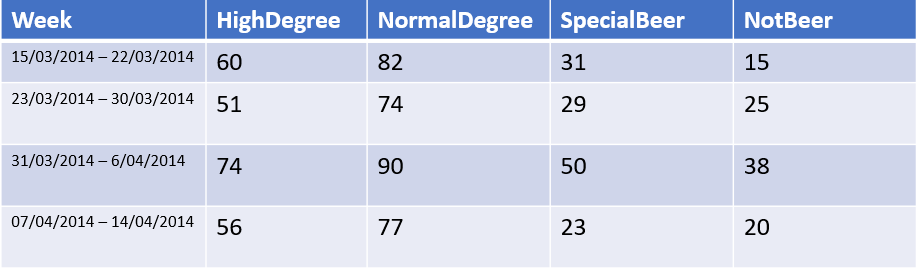
\includegraphics[scale = 0.8]{FormatTable}

\section{Features}

In order to do our prediction we thing about using the following features :
\begin{itemize}
\item Day before next holiday 
\item Day before next exam
\item Promotion Index
\item Day after exam or holiday ?
\item Day before next large event ?
\end{itemize}

We think that those are the main influences on whether people buy more or less drinks in a bar. We didn't include the two last ones on the model for the moment, we'll see if there are needed after the first series of tests.

\subsection{Holidays}

The holidays data is gather in a CSV file with 3 columns, Year, WeekNo and Holiday. If the week is a Holiday week then the holiday column contains a 1. If it's a work week then there is a 0. After thinking about it we decided to not only consider if the week is or isn't a holidays week but also count the number of week before the next holidays. Indeed we foresee that people tend to buy more in a Bar when a Holiday is near.
So the data given to the machine learning model will be the counter to the next holiday.

\subsection{Exams}

The Exams data is also gathered in a CSV file with 3 columns, Year, WeekNo and Exam, we actually combined it with the Holiday one for simplicity. If there is an Exam this week the Exam column contains a 1 and a 0 if not. As we did for the holidays what would interest us is a counter to the next exam. But in the case of exams we also want to transcript the possibility of several week of exams following each other. So our idea is to examine the 3following weeks and ponderate them (the first is more impactfull than the third one, with coefficient 3,2,1). 

\subsection{Promotion}

As told before we decided to add a coefficient that reflects the promotion ! Every promotion doesn't drink the same, a coefficient should be schoolyear based. So we just add a feature indicating the "promotion". We hope that the ML model will be able to consider the feature and balance the sales data of each year in accordance.

\vspace{5mm} 

Here is the final model of features that we will use for the first series of tests.

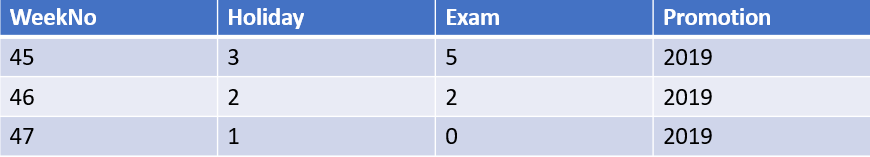
\includegraphics[scale=0.7]{DataModel}


\chapter{Model Selection}

Now the core of our work is to choose the best method to predict from our data. Or goal is to look in the dataset for features such as trends, cyclical fluctuations, seasonality, and behavioral patterns.


Here are the algorithm that we read about and could be used to forecast sales :
\begin{itemize}
\item KNN Regressor
\item Decision Tree
\item Random Forest
\item Neural network
\end{itemize}

We first use KNN and Decision which are simple to understand and analyze. 

\section{Finding the best Forecasting Method}

The goal is to compare the different models.

\subsection{First Results}

The first results are very disappointing, by using the KNN regressor and Decision Tree with different number of neighbors we find the following results :


\begin{figure}[!htb]
\minipage{0.32\textwidth}
  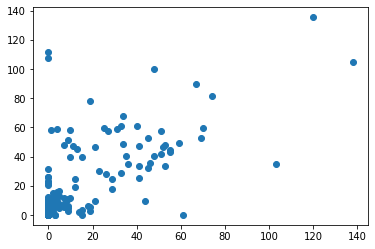
\includegraphics[width=\linewidth]{KNN5Nei.png}
  \caption{5 Neighbors}\label{fig:KNN5Nei}
\endminipage\hfill
\minipage{0.32\textwidth}
  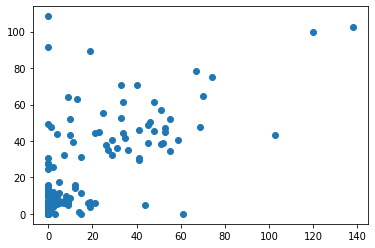
\includegraphics[width=\linewidth]{KNN10Nei.png}
  \caption{10 Neighbors}\label{fig:KNN10Nei}
\endminipage\hfill
\minipage{0.32\textwidth}%
  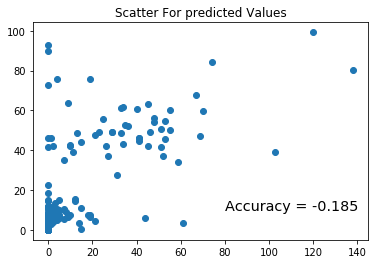
\includegraphics[width=\linewidth]{KNN20Nei.png}
  \caption{20 Neighbors}\label{fig:KNN20Nei}
\endminipage
\end{figure}


\begin{figure}[h!]
\centering
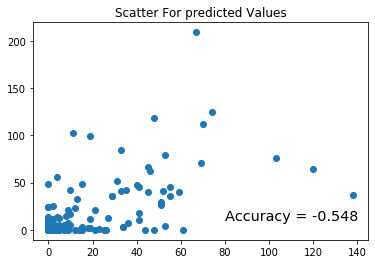
\includegraphics[scale=0.5]{DecisionTree}
\caption{Decision Tree}
\end{figure}


\section{Next Steps}

The accuracy results are very disappointing, our first thought is that the number of samples aren't sufficient, ie we don't have enough data. We actually have a lot of sales data, but as we gather it in weeks we have the equivalent of 8 (number of year considered) times 52 (weeks) samples. Maybe it isn't enough, we will have to dig in that issue. We think about reading other research with time series to see what is the range of data quantity necessary.
Other than date we will use Random Forest and try a Neural Network, which could be powerfull. 

\section{Individual Repartition}

\subsection{Maxime}

\begin{itemize}
\item Data Selection
\item Data extraction
\item Data Management and Sorting
\end{itemize}



\subsection{Mathieu}

\begin{itemize}
\item Research of models to use 
\item Adapt Data to use models
\item Analysis of first results
\end{itemize}


\section{Inspirations}

https://towardsdatascience.com/sales-forecasting-from-time-series-to-deep-learning-5d115514bfac : Forecasting principles and basis 

https://medium.com/analytics-vidhya/walmart-sales-forecasting-d6bd537e4904 : Forecasting at Walmart 

\section{GitHub}

Github link : https://github.com/Maxime-Michel-1999/BabarSalesForecast




\end{document}